\documentclass[xcolor=svgnames]{beamer}
%\documentclass[xcolor=svgnames,handout]{beamer}
\usetheme{Boadilla}
\usecolortheme[named=ForestGreen]{structure}
\usepackage{graphicx}
\usepackage[final]{animate}
%\usepackage[colorlinks=true,urlcolor=blue,citecolor=blue,linkcolor=blue]{hyperref}
\usepackage{breqn}
\usepackage{xcolor}
\usepackage{booktabs}
\usepackage{tikz}
\usetikzlibrary{shadows}
\usepackage[noae]{Sweave}
\definecolor{links}{HTML}{2A1B81}
\hypersetup{colorlinks,linkcolor=links,urlcolor=links}
\usepackage{pgfpages}
%\pgfpagesuselayout{4 on 1}[letterpaper, border shrink = 5mm, landscape]

\begin{document}
\Sconcordance{concordance:intro_to_R.tex:intro_to_R.Rnw:%
1 159 1 1 2 3 0 1 1 2 0 1 1 2 0 1 1 3 0 1 2 8 1 1 2 1 0 1 1 5 0 2 1 6 0 %
1 2 1 1 1 2 6 0 1 1 6 0 1 2 10 1 1 2 6 0 1 1 6 0 1 2 5 1 1 2 4 0 1 2 47 %
1}


\title[Intro to R]{Introduction to 
\includegraphics[width=0.07\textwidth]{Rlogo.jpg}}
\author[M. Beck and S. Berg]{Marcus W. Beck \and Sergey Berg}

\institute[UofM]{Department of Fisheries, Wildlife, and Conservation Biology \\ University of Minnesota, Twin Cities}

\date{May 21, 2013}

\titlegraphic{
\centerline{
\begin{tikzpicture}
  \node[drop shadow={shadow xshift=0ex,shadow yshift=0ex},fill=white,draw] at (0,0) {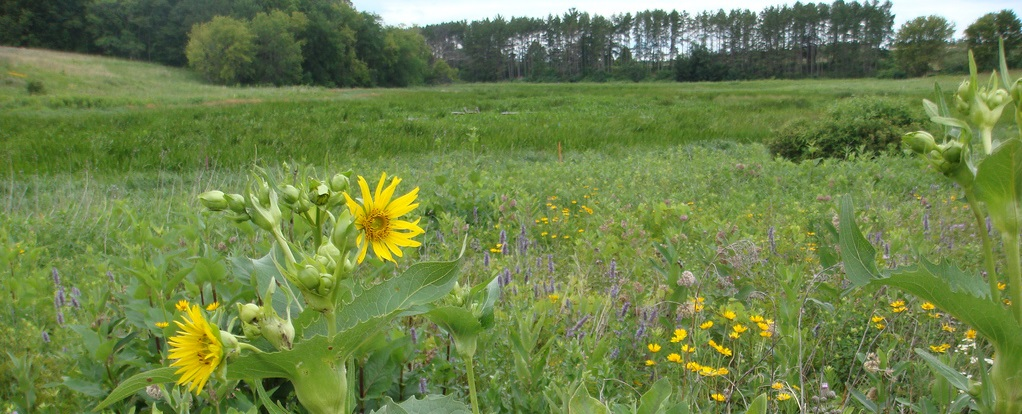
\includegraphics[width=0.6\textwidth]{peeper.jpg}};
\end{tikzpicture}}
}

%%%%%%
\begin{frame}
\vspace{-0.3in}
\titlepage
\end{frame}

%%%%%%
\begin{frame}{What you'll learn about \hspace{0.2em}
\includegraphics[width=0.07\textwidth]{Rlogo.jpg}}
\setbeamercovered{again covered={\opaqueness<1->{25}}}
\begin{itemize}
\itemsep15pt
\item What is R?
\item What's possible with R?
\item R basics
\begin{itemize}
\item Installation
\item Command-line interface
\item Coding basics
\end{itemize}
\item Help!\\~\\
\end{itemize}
\Large
\centerline{\emph{Interactive!}}
\end{frame}


\section{Background}

%%%%%%
\begin{frame}{What is 
\includegraphics[width=0.07\textwidth]{Rlogo.jpg} \hspace{0.2em}? }
\setbeamercovered{again covered={\opaqueness<1->{25}}}
R is a computer language that allows the user to program algorithms and use tools that
have been programmed by others [Zuur et al. 2009]\\~\\
Different from other statistics software because it is also a programming language...

\end{frame}

%%%%%%
\begin{frame}[t]{What is 
\includegraphics[width=0.07\textwidth]{Rlogo.jpg} \hspace{0.2em}? }
\vspace{-0.1in}
\begin{columns}
\begin{column}{0.4\textwidth}
R is becoming the statistical software of choice\\~\\
Plot of Google scholar hits over time for different software packages
[\href{http://r4stats.com/articles/popularity/}{r4stats.com}]
\end{column}
\begin{column}{0.5\textwidth}
\begin{center}
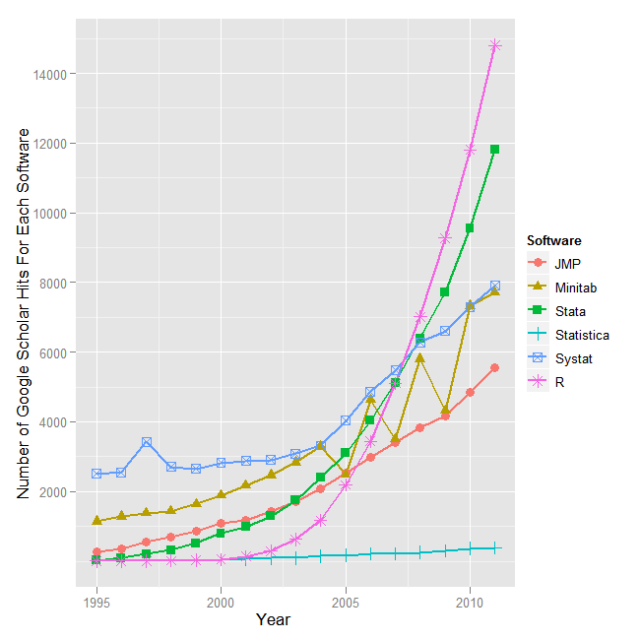
\includegraphics[width=1.1\textwidth]{r_google.png}
\end{center}
\end{column}
\end{columns}
\end{frame}

%%%%%%
\begin{frame}{What's possible with 
\includegraphics[width=0.07\textwidth]{Rlogo.jpg} \hspace{0.2em}? }
R is incredibly flexible, if you want something done, someone else has written the code...\\~\\
R is open-source software, which mean it's free and is supported by a large network of contributors - the Comprehensive R Network [\href{http://cran.us.r-project.org/}{CRAN}]\\~\\
Basically an online repository of R utilities that others have written
\end{frame}

% %%%%%%
% \begin{frame}[t,fragile]{What's possible with 
\includegraphics[width=0.07\textwidth]{Rlogo.jpg} \hspace{0.2em}? }
% <<eval=false,echo=true>>=
% demo(package = .packages(all.available = TRUE))
% @
% List of demonstrations with available packages - examples from ggplot2 package
% \begin{columns}
% \begin{column}{0.5\textwidth}
% \begin{center}
% 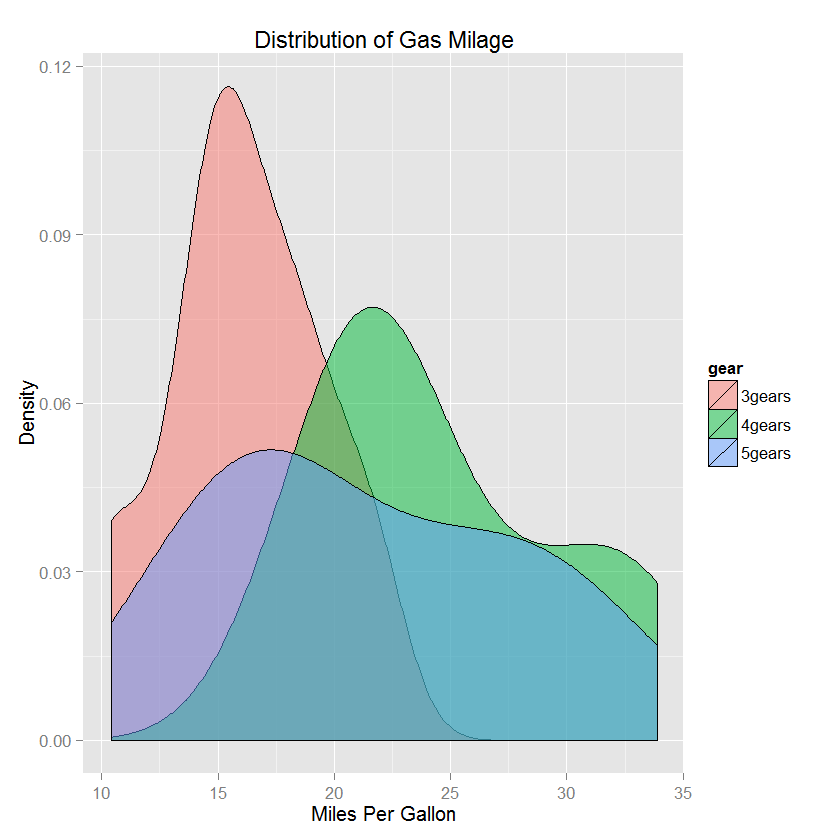
\includegraphics[width=\textwidth]{ggplot1.png}
% \end{center}
% \end{column}
% \begin{column}{0.5\textwidth}
% \begin{center}
% 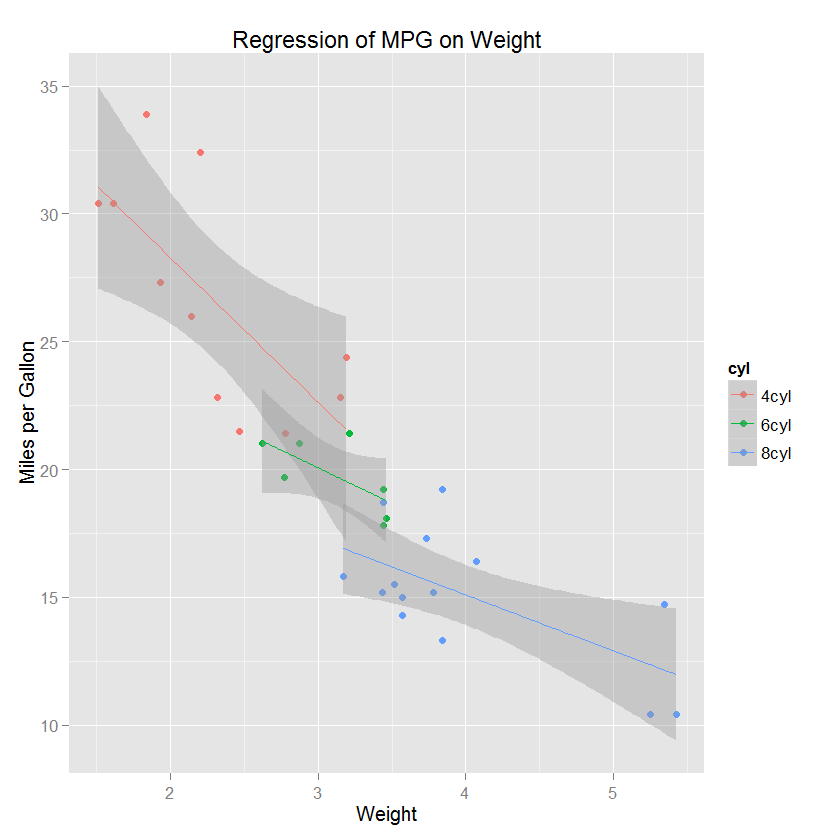
\includegraphics[width=\textwidth]{ggplot3.png}
% \end{center}
% \end{column}
% \end{columns}
% \end{frame}
% 
% %%%%%%
% \begin{frame}[t,fragile]{What's possible with 
\includegraphics[width=0.07\textwidth]{Rlogo.jpg} \hspace{0.2em}? }
% <<eval=false,echo=true>>=
% demo(package = .packages(all.available = TRUE))
% @
% List of demonstrations with available packages - examples from ggplot2 package
% \begin{columns}
% \begin{column}{0.5\textwidth}
% \begin{center}
% 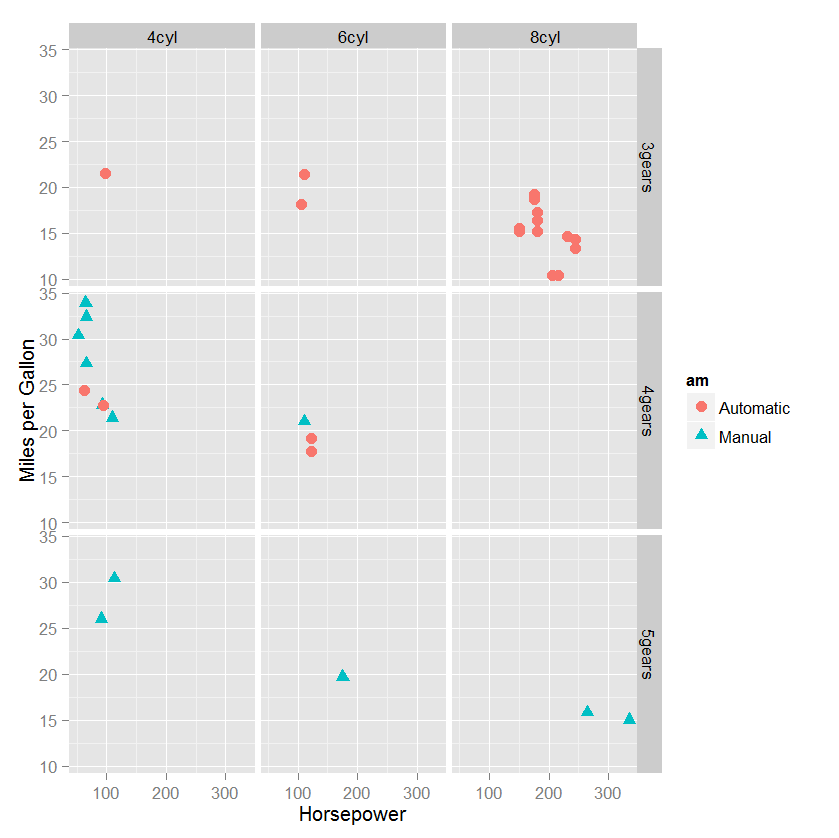
\includegraphics[width=\textwidth]{ggplot2.png}
% \end{center}
% \end{column}
% \begin{column}{0.5\textwidth}
% \begin{center}
% 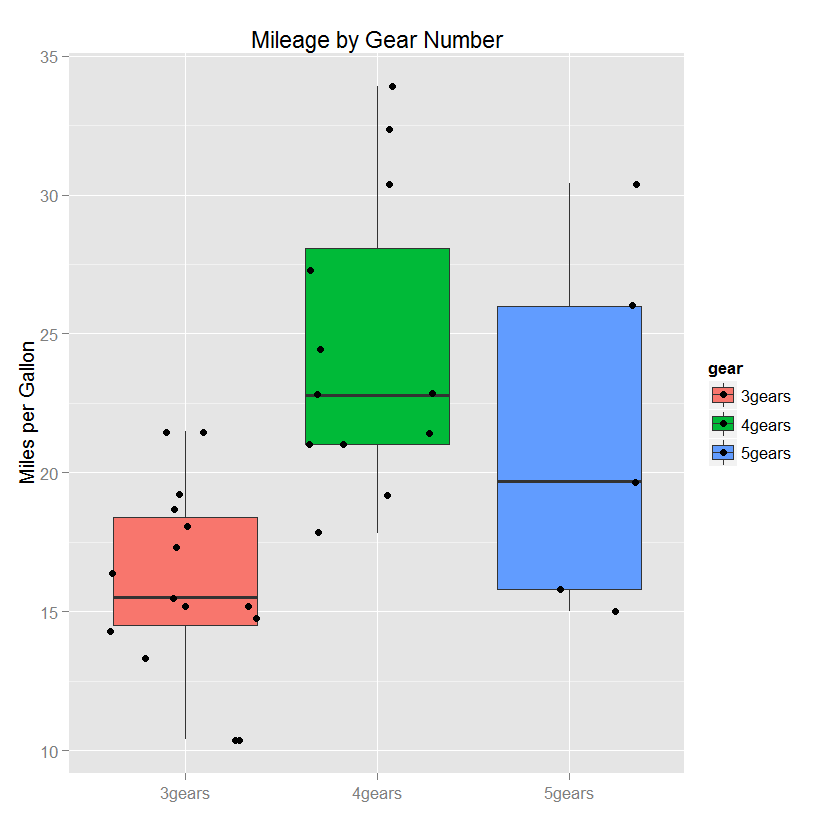
\includegraphics[width=\textwidth]{ggplot4.png}
% \end{center}
% \end{column}
% \end{columns}
% \end{frame}

\section{Basics}
%%%%%%
\begin{frame}[t]{
\includegraphics[width=0.07\textwidth]{Rlogo.jpg} \hspace{0.01in} basics}
Installation - visit \href{http://cran.us.r-project.org/}{r-project.org} and follow directions
\centerline{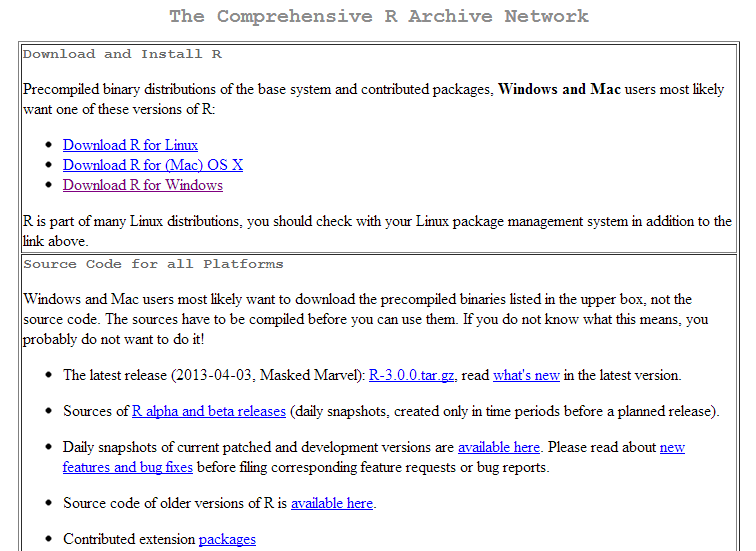
\includegraphics{download.png}}
\end{frame}

%%%%%%
\begin{frame}[t]{
\includegraphics[width=0.07\textwidth]{Rlogo.jpg} \hspace{0.01in} basics}
A text editor is highly recommended, e.g. \href{http://www.rstudio.com/}{RStudio}\\~\\
\centerline{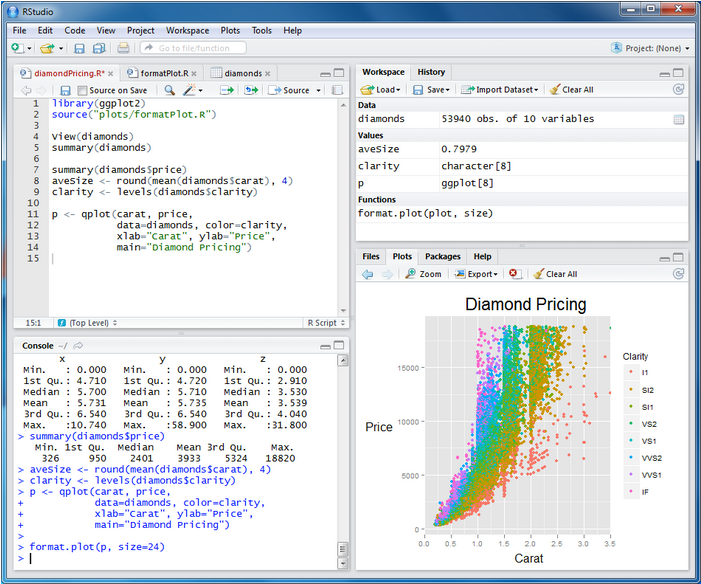
\includegraphics[width=0.65\textwidth]{Rstudio.png}}
\end{frame}

%%%%%%
\begin{frame}[t]{
\includegraphics[width=0.07\textwidth]{Rlogo.jpg} \hspace{0.01in} basics}
How is R different from Excel? R is a command-line interface\\~\\
\centerline{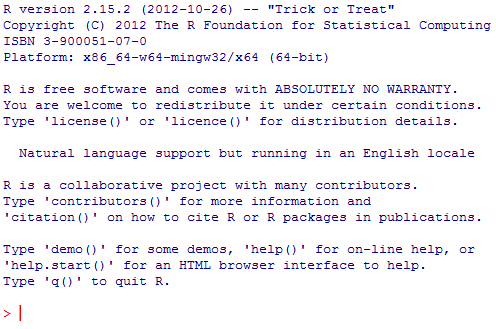
\includegraphics[width=0.7\textwidth]{command_line.png}}
\centerline{\emph{What next??}}
\end{frame}

%%%%%%
\begin{frame}[fragile]{
\includegraphics[width=0.07\textwidth]{Rlogo.jpg} \hspace{0.01in} basics}
Lines of code are executed by R at the prompt (\textit{\texttt{>}})\\~\\
Enter the code and press enter, the output is returned\\~\\
\begin{Schunk}
\begin{Sinput}
> print('hello world!')
\end{Sinput}
[1] "hello world!"\begin{Sinput}
> 2+2
\end{Sinput}
[1] 4\begin{Sinput}
> (2+2)/4
\end{Sinput}
[1] 1\begin{Sinput}
> rep("a",4)
\end{Sinput}
[1] "a" "a" "a" "a"\end{Schunk}

\end{frame}

%%%%%%
\begin{frame}[t,fragile]{
\includegraphics[width=0.07\textwidth]{Rlogo.jpg} \hspace{0.01in} basics}
Assigning data to R objects is critical for analysis\\~\\
Assignment is possible using \textit{\texttt{<-}} or \textit{\texttt{=}}\\~\\
\begin{columns}[t]
\begin{column}{0.5\textwidth}
\begin{Schunk}
\begin{Sinput}
> a<-2
> a
\end{Sinput}
\begin{Soutput}
[1] 2
\end{Soutput}
\begin{Sinput}
> b=3
> b
\end{Sinput}
\begin{Soutput}
[1] 3
\end{Soutput}
\end{Schunk}
\end{column}
\begin{column}{0.5\textwidth}
\begin{Schunk}
\begin{Sinput}
> a+1
\end{Sinput}
\begin{Soutput}
[1] 3
\end{Soutput}
\begin{Sinput}
> b*a
\end{Sinput}
\begin{Soutput}
[1] 6
\end{Soutput}
\end{Schunk}
\end{column}
\end{columns}
\end{frame}

%%%%%%
\begin{frame}[fragile]{
\includegraphics[width=0.07\textwidth]{Rlogo.jpg} \hspace{0.01in} basics}
Anatomy of a function - functions perform tasks for you, much like in Excel
\begin{center}
\Large
function(arguments)
\end{center}
\begin{Schunk}
\begin{Sinput}
> c(1,2) #concatenate function
\end{Sinput}
\begin{Soutput}
[1] 1 2
\end{Soutput}
\begin{Sinput}
> mean(c(1,2)) #mean function
\end{Sinput}
\begin{Soutput}
[1] 1.5
\end{Soutput}
\end{Schunk}
\end{frame}

%%%%%%
\begin{frame}[t,fragile]{
\includegraphics[width=0.07\textwidth]{Rlogo.jpg} \hspace{0.01in} basics}
How are data imported into R?\\~\\
R needs to know where the data are located on your computer:\\~\\
\begin{Schunk}
\begin{Sinput}
> setwd("C:/projects/my_data/")
\end{Sinput}
\end{Schunk}
\vspace{0.2in}
This establishes a `working directory' for data import/export\\~\\
R can import almost any type of data - usually not directly from Excel\\~\\
\end{frame}

% %%%%%%
% \begin{frame}[t,fragile]{
\includegraphics[width=0.07\textwidth]{Rlogo.jpg} \hspace{0.01in} basics}
% How are data imported into R?\\~\\
% R can import Excel data using the RODBC package, but this is not simple\\~\\
% \onslide<2>
% The easiest approach is to format data in Excel then export to a .csv or .txt file
% \begin{columns}
% \begin{column}{0.43\textwidth}
% \begin{center}
% 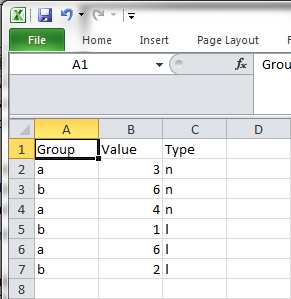
\includegraphics{my_dat.png}
% \end{center}
% \end{column}
% \begin{column}{0.66\textwidth}
% \begin{center}
% 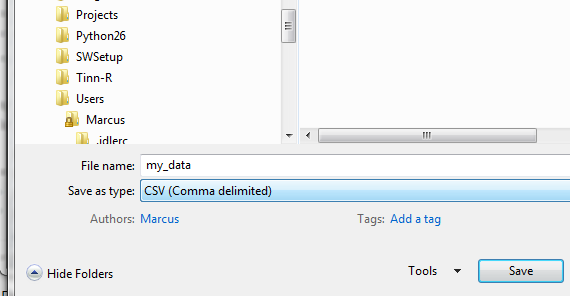
\includegraphics{save_as.png}
% \end{center}
% \end{column}
% \end{columns}
% \end{frame}

%%%%%%
\begin{frame}[t,fragile]{
\includegraphics[width=0.07\textwidth]{Rlogo.jpg} \hspace{0.01in} basics}
Where to go for help?\\~\\
\begin{itemize}
\addtolength{\itemsep}{0.08in}
\item A user-friendly \href{http://www.statmethods.net/}{intro to R} 
\item Several good introductory texts are available - Zuur et al. 2009. A Beginner's Guide to R. Springer.
\item \href{http://cran.r-project.org/doc/contrib/Short-refcard.pdf}{R cheatsheet}
\item Google is your friend 
\item Help files for each function using `?function' - may or may not be helpful 
\item An \href{http://cran.r-project.org/doc/manuals/R-intro.html}{intro to R} - very detailed
\item Ask us!
\end{itemize}
\end{frame}

% \begin{frame}[shrink]{References}%[t,allowframebreaks]{References}
% \scriptsize
% \setbeamertemplate{bibliography item}{}
% \bibliographystyle{C:/Projects/LaTeX/bibtex_bst/apalike_mine}
% \bibliography{C:/Projects/LaTeX/ref_diss}
% \end{frame}

\end{document}
